% type et packages %%%%%%%%%%%%%%%%%%%%%%%%%%%%%%%%%%%%%%%%%%%%%%%%%%%%%%%%%%%%%%%%%%%%%%%%%%%
\documentclass{report}

\usepackage[utf8]{inputenc} % un package
\usepackage[T1]{fontenc}      % un second package
\usepackage[francais]{babel}  % un troisième package
\usepackage{graphicx}
\usepackage{float}
\usepackage{ccicons}
\usepackage{url}
\usepackage{amsmath,amsfonts,amssymb}
\usepackage{pgfplots}
\usepackage{wasysym}
\usepackage{braket}
\usepackage{listings}
\usepackage{sagetex}

\usepackage[europeanvoltages, europeancurrents, europeanresistors, americaninductors]{circuitikz}

\def\releaseversion{1} %Mettre à 1 pour afficher les graphiques


% en-tête et pied de page %%%%%%%%%%%%%%%%%%%%%%%%%%%%%%%%%%%%%%%%%%%%%%%%%%%%%%%%%%%%%%%%%%%%
\usepackage{fancyhdr}
\usepackage[headheight = 2cm,bottom=3.5cm]{geometry}
\pagestyle{fancy}
\renewcommand{\headrulewidth}{1pt}
\fancyhead[L]{
\includegraphics[height=1.5cm]{icestudio.png}} 
\fancyhead[C]{\textsc{Icestudio ``filtering'' documentation\\}}
\fancyhead[R]{}
\renewcommand{\footrulewidth}{1pt}
\fancyfoot[C]{Baptiste LEGOUIX - 1.0, December 2017} 
\fancyfoot[L]{\huge \ccLogo \ccZero}
\fancyfoot[R]{\thepage}

\makeatletter
\let\ps@plain\ps@fancy
\makeatother

% Document %%%%%%%%%%%%%%%%%%%%%%%%%%%%%%%%%%%%%%%%%%%%%%%%%%%%%%%%%%%%%%%%%%%%%%%%%%%%%%%%%%%

\begin{document}

This document has for aim to help Icestudio users to make a numerical filter working, and gives developers some informations about what has already been made and what still needs work.

I'm not expert in signal processing and HDL, then I don't plan to improve and extend this library in short-term. Do not hesitate to take over this project as you wish if you have the skills.

\section*{Filtering theory}

The Laplace-transform of a signal $f$ is given by :

\[
\mathcal{L}(f) : p \rightarrow \braket{f|e^{-p^*x}} = \int_\mathbb{R} f(x)e^{-p x} dx
\]

Where $p$ is a complex number. An important property is :

\[
\mathcal{L}\left(\frac{df}{dt} \right) = pf
\]

A filter $h$ is a signal-processing system which describes an ordinary differential equation, and can also be wrote as a Laplace transform (which is an algebric function).

When the differential equation is linear, its Laplace transform is a rationnal fraction. For example, a first-order low-pass :

\[
\frac{dy}{dt} + \frac{y}{\tau} = \frac{x}{\tau}
\]

\[
\mathcal{L}(h) : p \rightarrow \frac{1}{1 + \tau p}
\]

However, for numerical computing applications as FPGA it's better tu use z-transform which is closer to hardware. The idea is to consider a discretized signal $f$ where :

\[
f_{i+j} = z^j f_i
\]

Now, we need an integration method. The simplest is the Newton one :

\[
\frac{df}{dt} = \frac{f_i-f_{i-1}}{T_e}
\]

In the frequency-domain :

\[
p = \frac{1-z^{-1}}{T_e}
\]

Which gives a way to obtain z-transform knowing Laplace transform. For our first-order filter example :

\[
\mathcal{Z}(h)(z) = \frac{1}{1 + \tau \frac{1-z^{-1}}{T_e}}
\]

\[
\mathcal{Z}(h)(z) = \frac{1}{1+\frac{\tau}{T_e} - \frac{\tau}{T_e}z^{-1}}
\]

\[
\mathcal{Z}(h)(z) = \frac{\frac{1}{1+\frac{\tau}{T_e}}}{1 - \frac{\frac{\tau}{T_e}}{1+\frac{\tau}{T_e}}z^{-1}}
\]

Where $T_e$ is the sampling time (the clock period). We will place ourselves in a unit time-system in which $T_e=1$, but for concretes application you'll have to take it into account.

\[
\mathcal{Z}(h)(z) = \frac{\frac{1}{1+\tau}}{1 - \frac{\tau}{1+\tau}z^{-1}}
\]

Another commonly-used integration method is the Tustin one, which corresponds to :

\[
z = \frac{1+p\frac{T_e}{2}}{1-p\frac{T_e}{2}}
\]

If we use this method, we'll find another z-transform for the same continuous filter, but quite close in their coefficients.

Finally, we'll distinguish two sorts of numerical filters :

\begin{itemize}
\item Finite impulse response filters :

\[
\mathcal{Z}(h)(z) = \sum_{i=0}^\infty a_i z^{-i}
\]

\item Infinite impulse response filters :

\[
\mathcal{Z}(h)(z) = \frac{\sum_{i=0}^\infty b_i z^{-i}}{1+\sum_{i=1}^\infty a_i z^{-i}}
\]

\end{itemize}

\section*{Implementation}

Numbers must be coded in a signed fixed-point formats, on $n$ bits (I think \emph{yosys} doesn't support \emph{real} Verilog type). All blocks have a \emph{width} parameter which must be affected to $n\leq 64$.

Clocks are chained to generate positive edge when the task of a block takes end and the output register is filled ; then, the next block can begin.

Overflow isn't handled. Take care.

\subsection*{$z^{-1}$ block}

Remember that $z^j f_i = f_{i+j}$.

So, $z^{-1}$ is a simple register which delays the signal by one clock period :

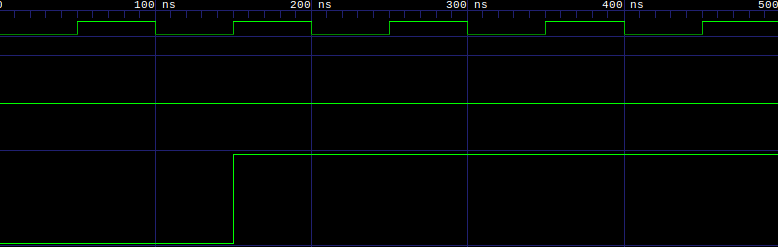
\includegraphics[width=\textwidth]{images/zminus1.png}

\subsection*{gain block}

This block multiply the input by the parameter $K$ :

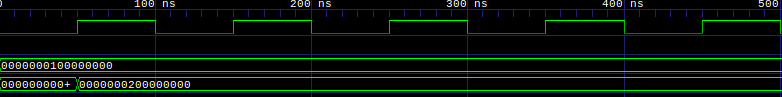
\includegraphics[width=\textwidth]{images/gain.png}

\subsection*{add block}

This block makes the sum of the inputs $a$ and $b$.

\subsection*{filteringcell block}

This is the core of all linear filtering structure. It's composed of one of each precedents blocks, and the value of the gain corresponds to one coefficient in a z-transform.

\subsection*{FIR blocks}

A first-order and a second-order FIR are availables. Pure derivative is obtained for $b_0=1$ and $b_1=-1$ :

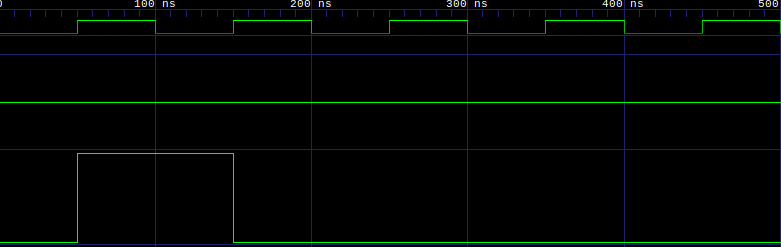
\includegraphics[width=\textwidth]{images/derivative.png}

Indeed, derivative of a step is a Dirac impulse.

These blocks are simples chains of \emph{filteringcell}s, whose the number corresponds to the order of the filter. I think we should propose a block with the order in parameter, but I don't know how to make it in Verilog.

\subsection*{IIR block}

This block makes use of two FIR filters to build an IIR (two-poles, two-zeros). Let's start with the integrator ($b_0=1$ and $a_1=-1$) :

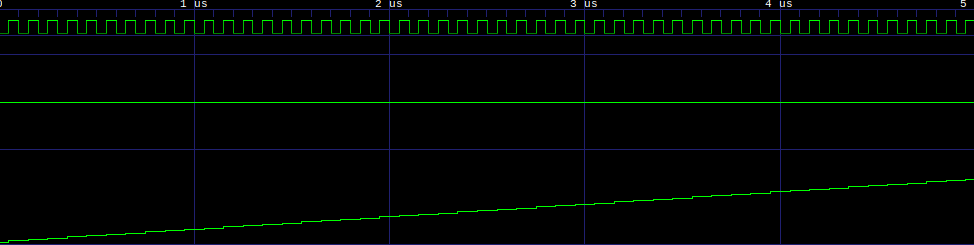
\includegraphics[width=\textwidth]{images/integration.png}

The following picture is the step response of the first order we took in example. I took $\tau = 10$, which corresponds to $b_0 = \frac{1}{1+\tau} = 0.1$ and $a_1 = -\frac{\tau}{1+\tau} = -0.9$ :

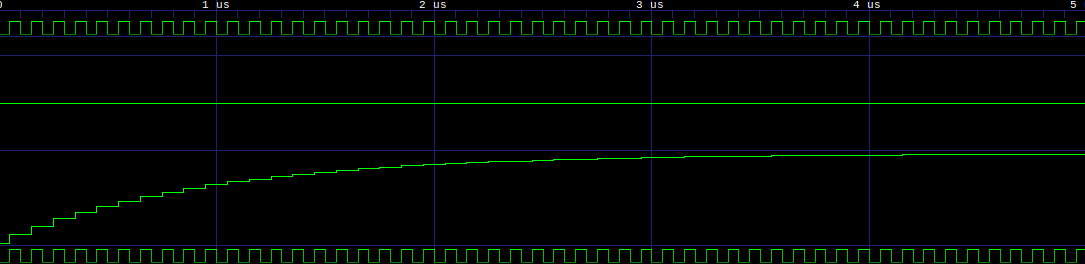
\includegraphics[width=\textwidth]{images/firstordertau10.png}

Same thing for the high-pass, which has the same setup except $b_1 = -\frac{1}{1+\tau} = -0.1$ :

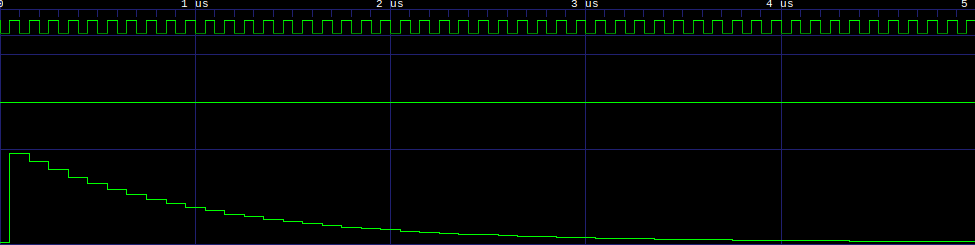
\includegraphics[width=\textwidth]{images/highpasstau10.png}

For another example, we'll take the following Laplace-transform (whose order is $2$) :

\[
\mathcal{L}(h)(p) = \frac{1}{1 + \frac{p}{Q\omega_0} + \frac{p^2}{\omega_0^2}}
\]

With $Q = 2$ ans $\omega_0 = 20\pi$, the theorical step response is :

\begin{sagesilent}
x=var('x');
t = var('t');
x_coords = [t for t in srange(0,2,0.01)];

x = var('x');
p = var('p');
w0 = 2*pi; Q = 2; v(x) = inverse_laplace(1/p/(1+p/Q/w0+p^2/w0^2), p, x);

y5_coords = [v(x).n() for x in x_coords];

output = "";
for i in range(0,len(x_coords)-1):
    output += "\draw[orange, thick] ("+str(x_coords[i])+","+str(y5_coords[i])+")--("+str(x_coords[i+1])+","+str(y5_coords[i+1])+");\n";
\end{sagesilent}

\begin{center}
\begin{tikzpicture}[x=5\textwidth/6/2), y=\textwidth/3/1.5]
 // Axes
 \draw[->] (0,0) -- (2.2,0) node[right] {$t$};
 \draw[->] (0,0) -- (0,1.5) node[above] {$y(t)$};
 //Graduation angulaire
 \foreach \x in {1,...,2}
      \draw (\x,0.03) -- (\x,-0.03)
  node[anchor=north] {$\x0$};
  
 \draw (0,0.95) node[left] {};
 \draw[dotted] (0,0.95) -- ++(2,0);
 \draw (0,1) node[left] {$1$};
 \draw[dotted] (0,1) -- ++(2,0);
 \draw (0,1.05) node[left] {};
 \draw[dotted] (0,1.05) -- ++(2,0);
	
 \draw (0.42,1.32) node[anchor=west] {\textcolor{orange}{$Q=2$}};
 \if\releaseversion1
 \sagestr{output}
 \fi
\end{tikzpicture}
\end{center}

With the substitution $p=1-z^{-1}$, we'll find :

\[
\mathcal{L}(h)(p) = \frac{\frac{1}{1 + \frac{1}{Q\omega_0} + \frac{1}{\omega_0^2}}}{1 
-\frac{\frac{1}{Q\omega_0} + \frac{2}{\omega_0^2}}{1 + \frac{1}{Q\omega_0} + \frac{1}{\omega_0^2}}z^{-1} 
+ \frac{\frac{1}{\omega_0^2}}{1 + \frac{1}{Q\omega_0} + \frac{1}{\omega_0^2}}z^{-2}}
\]

Which allows to calculate the coefficients :

\[
\left\{\begin{matrix}
b_0 = 0.0094 \\
a_1 = -1.934 \\
a_2 = 0.9434
\end{matrix}\right.
\]

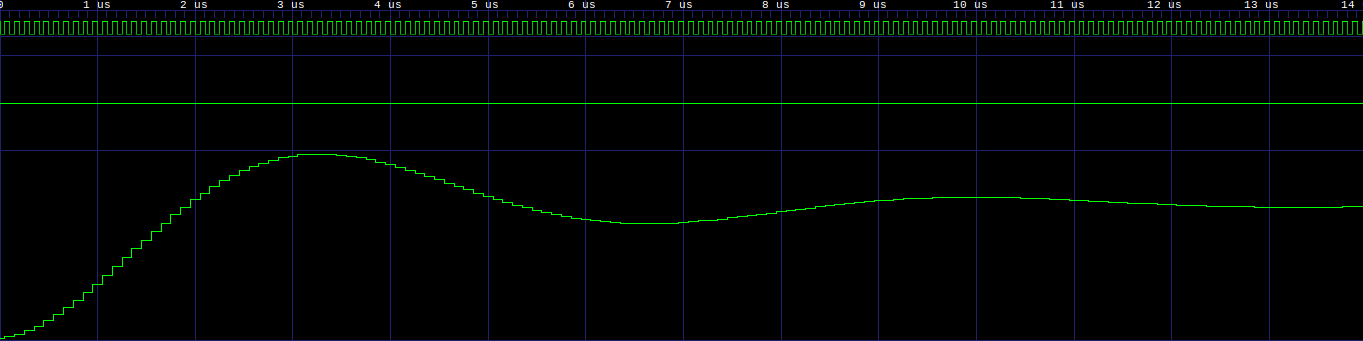
\includegraphics[width=\textwidth]{images/secondorderQ2f10.png}

\end{document}